\documentclass{report}

\usepackage[a4paper, left=1in, right=1in, top=1in, bottom=0.5in,]{geometry}
\usepackage{graphicx}
\usepackage{float}

\title{\Huge{Guessing Game Documentation}}
\author{\Huge{Suman Debnath \vspace{7mm}}}
\date{\Large{16-11-2022 \hspace{2mm} - \hspace{2mm} 21-11-2022}}

\begin{document}

\maketitle

\begin{center}
	\textsc{\LARGE{Objectives of Project}} 
\end{center}

\hfill

The objective of the project is to create a number-guessing game that takes numbers as user inputs and checks whether the input number matches the number chosen by the computer. If not, the computer provides hints to find the number, and finally if the number of tries runs out it prints the number else if the user manages to find the number, the player wins the game, and the computer prints out a greeting message. 

\hfill

\begin{center}
	\textsc{\LARGE{Function Description}}
\end{center}

\hfill

\begin{flushleft}
\texttt{init()}
\textsf{ : }
\end{flushleft}
\begin{flushright}
\hfill\begin{minipage}{0.85\linewidth}
	\textsf{		It initializes 'low' and 'high' integer variables to 0. It is used at the beginning of the 'play()' function.} \\ \\
	\textsf{parameters : }
	\texttt{none} \\ \\
	\textsf{return value: }
	\texttt{none}	\\ \\
\end{minipage}
\end{flushright}

\begin{flushleft}
\texttt{chooseGameMode()}
\textsf{ : }
\end{flushleft}
\begin{flushright}
\hfill\begin{minipage}{0.85\linewidth}
	\textsf{		It prints the three game modes available and takes input corresponding to the game mode from the user. } \\ \\
	\textsf{parameters : }
	\texttt{none} \\ \\
	
	\textsf{return value: }
	\texttt{int tries }	\\
	\textsf{ Returns the number of tries corresponding to the game mode. }\\ \\
\end{minipage}
\end{flushright}

\begin{flushleft}
\texttt{choose()}
\textsf{ : }
\end{flushleft}
\begin{flushright}
\hfill\begin{minipage}{0.85\linewidth}
	\textsf{		It assigns a random number to 'ranum' variable and prints a message when the number is chosen.} \\ \\
	\textsf{parameters : }
	\texttt{none} \\ \\
	\textsf{return value: }
	\texttt{void} \\ \\
\end{minipage}
\end{flushright}

\begin{flushleft}
\texttt{isVerified()}
\textsf{ : }
\end{flushleft}
\begin{flushright}
\hfill\begin{minipage}{0.85\linewidth}
	\textsf{		It checks whether the string input is numeric and then checks whether the numeric value is within the input limits according to the game mode.} \\ \\
	\textsf{parameters : }
	\texttt{char raw[]} \\ 
	\textsf{Raw is a string that contains the string form of the number entered by the user during gameplay} \\ \\
	\textsf{return value: }
	\texttt{int} \\
	\textsf{Returns 1 if the number is within the game mode limits else returns 0} \\ \\
\end{minipage}
\end{flushright}

\break

\begin{flushleft}
\texttt{decide()}
\textsf{ : }
\end{flushleft}
\begin{flushright}
\hfill\begin{minipage}{0.85\linewidth}
	\textsf{		It initializes 'low' and 'high' integer variables to 0. It is used at the beginning of the 'play()' function.} \\ \\
	\textsf{parameters : }
	\texttt{char raw\_input[],		int randum, 	int triess} \\ 
	\textsf{raw\_input contains the string form of input number. randum contains the value of ranum variable (random number). triess contains the value of tries variable (the number of tries).} \\ \\
	\textsf{return value: }
	\texttt{void} \\ \\
\end{minipage}
\end{flushright}


\begin{flushleft}
\texttt{play()}
\textsf{ : }
\end{flushleft}
\begin{flushright}
\hfill\begin{minipage}{0.85\linewidth}
	\textsf{		It is the method that runs the gameplay. It runs init() and choose() and then ask the user for the number inputs. Then it runs isVerified() to check whether the entered input is valid or not. If the input is valid it checks whether the input matches with number chosen by computer and prints out the according message. When the number of tries run out it prints the number chosen by the computer. If the input number matches the number chosen by computer the player wins and the a greeting message is printed out. Then the player is provided with an option to replay the game or quit.} \\ \\
	\textsf{parameters : }
	\texttt{none} \\ \\
	\textsf{return value: }
	\texttt{void} \\ \\
\end{minipage}
\end{flushright}

\hfill

\begin{center}
	\textsc{\LARGE{Profiling Report}}
\end{center}

\hfill

\begin{verbatim}

Flat profile:

Each sample counts as 0.01 seconds.
 no time accumulated

  %   cumulative   self              self     total           
 time   seconds   seconds    calls  Ts/call  Ts/call  name    

 %         the percentage of the total running time of the
time       program used by this function.

cumulative a running sum of the number of seconds accounted
 seconds   for by this function and those listed above it.

 self      the number of seconds accounted for by this
seconds    function alone.  This is the major sort for this
           listing.

calls      the number of times this function was invoked, if
           this function is profiled, else blank.

 self      the average number of milliseconds spent in this
ms/call    function per call, if this function is profiled,
	   else blank.

 total     the average number of milliseconds spent in this
ms/call    function and its descendents per call, if this
	   function is profiled, else blank.

name       the name of the function.  This is the minor sort
           for this listing. The index shows the location of
	   the function in the gprof listing. If the index is
	   in parenthesis it shows where it would appear in
	   the gprof listing if it were to be printed.

Copyright (C) 2012-2022 Free Software Foundation, Inc.

Copying and distribution of this file, with or without modification,
are permitted in any medium without royalty provided the copyright
notice and this notice are preserved.

		     Call graph (explanation follows)


granularity: each sample hit covers 4 byte(s) no time propagated

index % time    self  children    called     name

 This table describes the call tree of the program, and was sorted by
 the total amount of time spent in each function and its children.

 Each entry in this table consists of several lines.  The line with the
 index number at the left hand margin lists the current function.
 The lines above it list the functions that called this function,
 and the lines below it list the functions this one called.
 This line lists:
     index	A unique number given to each element of the table.
		Index numbers are sorted numerically.
		The index number is printed next to every function name so
		it is easier to look up where the function is in the table.

     % time	This is the percentage of the `total' time that was spent
		in this function and its children.  Note that due to
		different viewpoints, functions excluded by options, etc,
		these numbers will NOT add up to 100%.

     self	This is the total amount of time spent in this function.

     children	This is the total amount of time propagated into this
		function by its children.

     called	This is the number of times the function was called.
		If the function called itself recursively, the number
		only includes non-recursive calls, and is followed by
		a `+' and the number of recursive calls.

     name	The name of the current function.  The index number is
		printed after it.  If the function is a member of a
		cycle, the cycle number is printed between the
		function's name and the index number.


 For the function's parents, the fields have the following meanings:

     self	This is the amount of time that was propagated directly
		from the function into this parent.

     children	This is the amount of time that was propagated from
		the function's children into this parent.

     called	This is the number of times this parent called the
		function `/' the total number of times the function
		was called.  Recursive calls to the function are not
		included in the number after the `/'.

     name	This is the name of the parent.  The parent's index
		number is printed after it.  If the parent is a
		member of a cycle, the cycle number is printed between
		the name and the index number.

 If the parents of the function cannot be determined, the word
 `<spontaneous>' is printed in the `name' field, and all the other
 fields are blank.

 For the function's children, the fields have the following meanings:

     self	This is the amount of time that was propagated directly
		from the child into the function.

     children	This is the amount of time that was propagated from the
		child's children to the function.

     called	This is the number of times the function called
		this child `/' the total number of times the child
		was called.  Recursive calls by the child are not
		listed in the number after the `/'.

     name	This is the name of the child.  The child's index
		number is printed after it.  If the child is a
		member of a cycle, the cycle number is printed
		between the name and the index number.

 If there are any cycles (circles) in the call graph, there is an
 entry for the cycle-as-a-whole.  This entry shows who called the
 cycle (as parents) and the members of the cycle (as children.)
 The `+' recursive calls entry shows the number of function calls that
 were internal to the cycle, and the calls entry for each member shows,
 for that member, how many times it was called from other members of
 the cycle.

Copyright (C) 2012-2022 Free Software Foundation, Inc.

Copying and distribution of this file, with or without modification,
are permitted in any medium without royalty provided the copyright
notice and this notice are preserved.

Index by function name

\end{verbatim}

\break

\hfill

\begin{center}
	\textsc{\LARGE{Debugging Report}}
\end{center}

\hfill

\begin{figure}[H]
  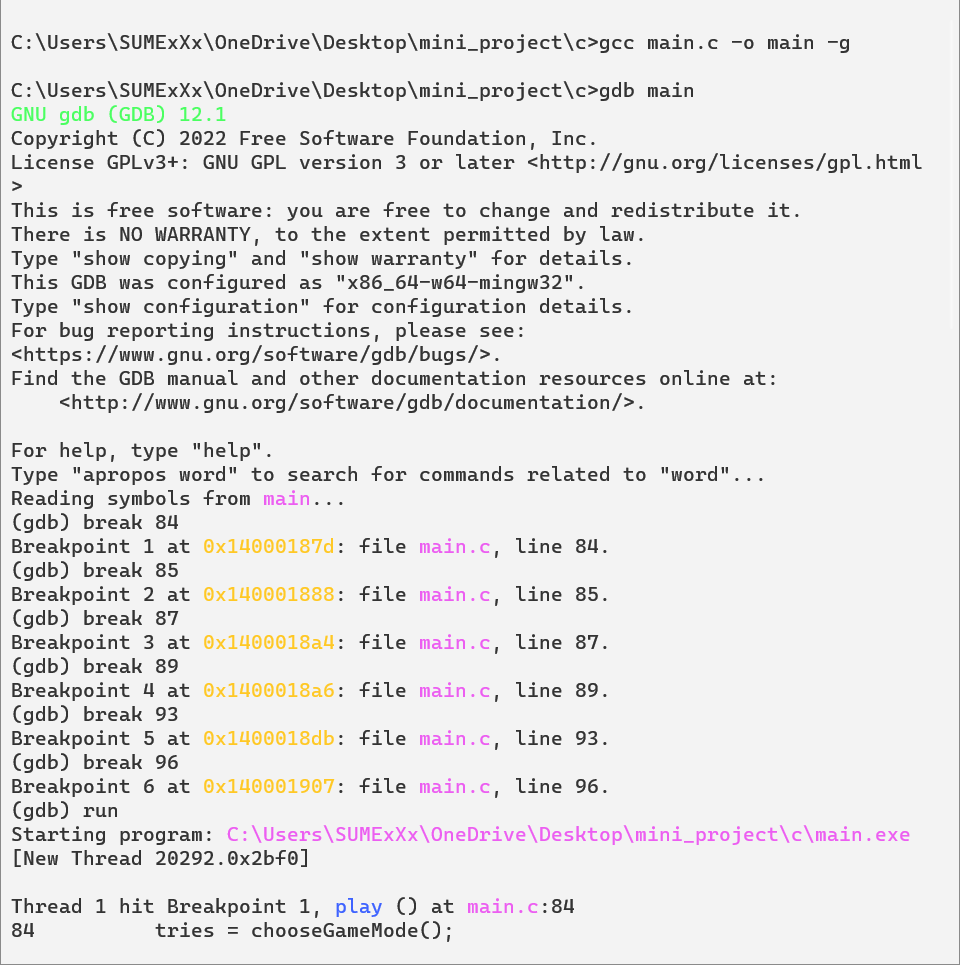
\includegraphics[width=\linewidth]{pic1.png}
  \caption{Screenshot of debugging report}
  \label{Debug picture 1}
\end{figure}

\begin{figure}[H]
  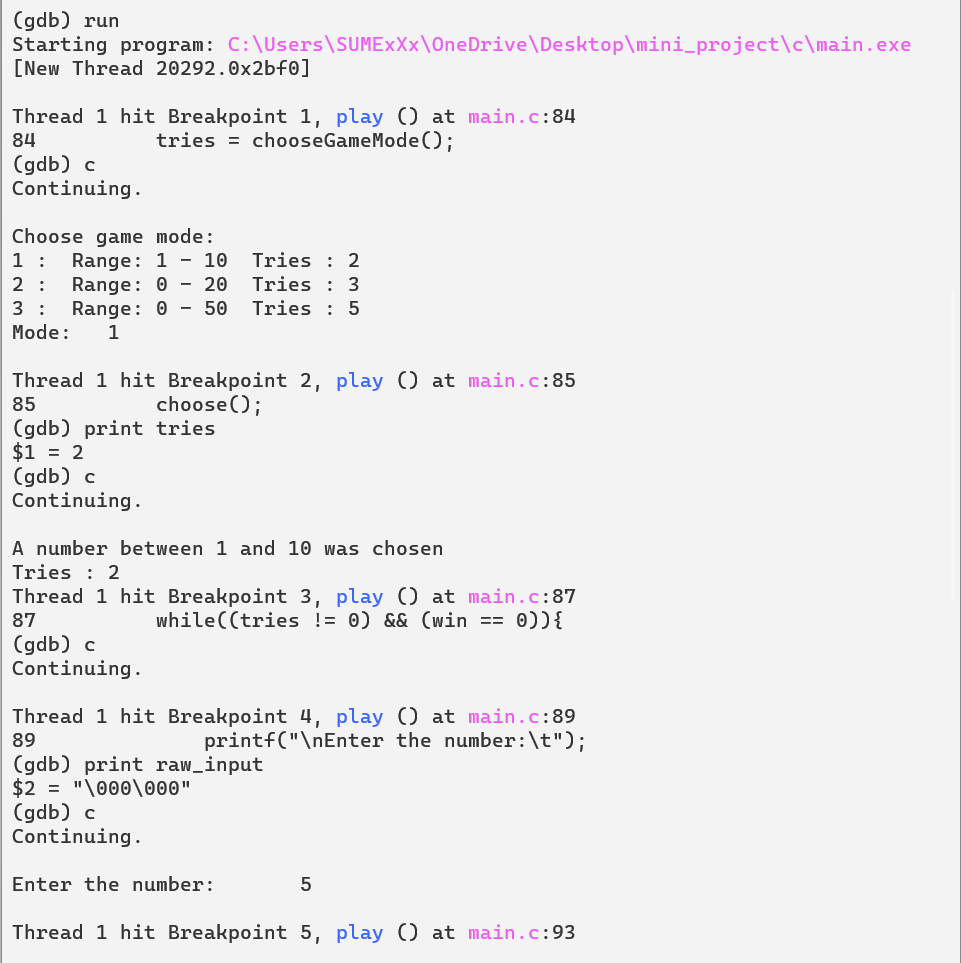
\includegraphics[width=\linewidth]{pic2.png}
  \caption{Screenshot of debugging report}
  \label{Debug picture 2}
\end{figure}

\begin{figure}[H]
  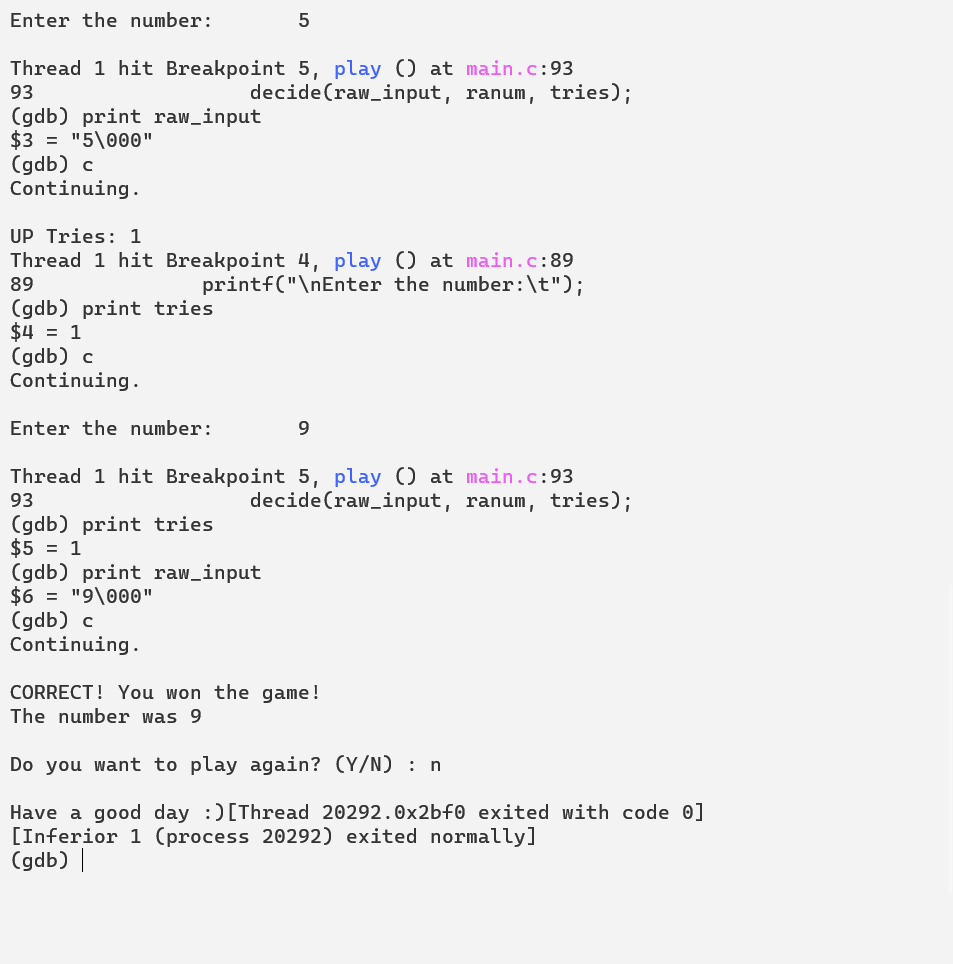
\includegraphics[width=\linewidth]{pic3.png}
  \caption{Screenshot of debugging report}
  \label{Debug picture 3}
\end{figure}

\hfill

\break

\begin{center}
	\textsc{\LARGE{Code in C Language}}
\end{center}

\begin{verbatim}

#include <stdio.h>
#include <stdlib.h>
#include <string.h>
#include <time.h>

int low;
int high;
int ranum;
int mode;
int tries;
int win;

// This function initialises the 'high' and 'mode' variables
// It takes no parameter and returns nothing.

void init(){
    low = 10;
    high = 60;
}

// This function prints the details of the three game modes and asks the 
//user to input 1 for 1st game mode, 2 for 2nd game mode and 3 for
// 3rd game mode.    It takes no parameter and returns the value of tries variable

int chooseGameMode(){

    printf("\nChoose game mode:\n1 :  Range: 1 - 10  Tries : 2\n2 :  Range: 
0 - 20  Tries : 3\n3 :  Range: 0 - 50  Tries : 5\nMode:\t");
    scanf("%d", &mode);

    if(mode == 1){
        tries = 2;
        low = 1;
        high = 11;
        return 2;
    }else if(mode == 2){
        tries = 3;
        low = 1;
        high = 21;
        return 3;
    }else if(mode == 3){
        tries = 5;
        low = 1;
        high = 51;
        return 5;
    }else {
        printf("\nWrong input");
        chooseGameMode();
    }
}

// This function picks a random number between the range [low, high] and 
// assigns it to the variable 'ranum'

void choose(){
    srand(time(0));
    ranum = (rand() % (high - low)) + low;
    printf("\nA number between %d and %d was chosen",low, high-1);
}

// This function verifies whether the supplied string 'raw' is numeric or not and
// then it checks whether the numeric value of raw is in between
// low and high.     It takes three parameter : raw and returns 1 or 0

int isVerified(char raw[]){

    int value = atoi(raw);
    if((value>= low) && (value<high)){
        return 1;
    }else{
        return 0;
    }
}

// This function checks whether the raw_input (the numeric value) supplied by 
// user is equal to the random number (ranum)
// or less or greater than ranum and also checks whether the number of tries 
//left or not prints the message accordingly
// ("Correct!", "UP" and "DOWN").    It takes three parameter : raw_input, randum,
// tries and returns nothing.

void decide(char raw_input[], int randum, int triess) {
    char stat[10];
    win = 0;
    if (atoi(raw_input) == randum) {
        strcpy(stat, "CORRECT!");
        win = 1;

    } else if (atoi(raw_input) < randum) {
        strcpy(stat, "UP");
    } else {
        strcpy(stat, "DOWN");
    }

    if ((triess > 1) && (win == 0)) {
        printf("\n%s Tries: %d", stat, tries - 1);
    }

    if (win == 1){
        printf("\n%s You won the game!", stat);
    }
}

// This function is the entry point for the program. It contains init(),
// chooseGameMode(), choose() in order and then it takes input from
// user and runs isVerified() and decide() in a loop till the tries variable 
// become 0. Then it exits out of the loop
// and asks the user whether to replay or not. Finally it prints "Have a good day :)"

void play(){
    init();
    tries = chooseGameMode();
    choose();
    printf("\nTries : %d", tries);
    while((tries != 0) && (win == 0)){
        char raw_input[3];
        printf("\nEnter the number:\t");
        scanf("%s", raw_input);

        if(isVerified(raw_input)){
            decide(raw_input, ranum, tries);
            tries -= 1;
        }else{
            printf("\nWrong input, try again");
        }
    }
    printf("\nThe number was %d", ranum);

    char inp;
    printf("\n\nDo you want to play again? (Y/N) : ");
    fflush(stdin);
    scanf("%c", &inp);

    if ((inp == 'Y') || (inp == 'y')){
        play();
    }else{
        printf("\nHave a good day :)");
    }
}

int main() {
    play();
    return 0;
}
\end{verbatim}

\hfill

\begin{center}
	\textsc{\LARGE{Output of Code in C Language}}
\end{center}

\hfill

\begin{verbatim}
Choose game mode:
1 :  Range: 1 - 10  Tries : 2
2 :  Range: 0 - 20  Tries : 3
3 :  Range: 0 - 50  Tries : 5
Mode:2

A number between 1 and 20 was chosen
Tries : 3
Enter the number:10

DOWN Tries: 2
Enter the number:5

DOWN Tries: 1
Enter the number:2

The number was 1

Do you want to play again? (Y/N) :n

Have a good day :)
Process finished with exit code 0
\end{verbatim}

\hfill

\break

\begin{center}
	\textsc{\LARGE{Code in Python Language}}
\end{center}

\hfill

\begin{verbatim}
import numpy as np

# This function initialises the 'runum', 'tries', 'low', 'high', 'mode' and 'win' variables
# It takes no parameter and returns nothing.

def init():
    global ranum
    global tries
    global low
    global high
    global mode
    global win
    win = 0
    low = 10
    high = 60

# This function prints the details of the three game modes and asks the user to 
#input 1 for 1st game mode, 2 for 2nd game mode and 3 for
# 3rd game mode.    It takes no parameter and returns the value of tries variable

def chooseGameMode():
    global mode
    global tries
    global low
    global high

    mode = int(input("\nChoose game mode:\n1 :  Range: 1 - 10  Tries : 2\n2 :  
Range: 0 - 20  Tries : 3\n3 :  Range: 0 - 50  Tries : 5\nMode: "))
    if mode == 1:
        tries = 2
        low = 1
        high = 11
        return 2
    elif mode == 2:
        tries = 3
        low = 1
        high = 21
        return 3
    elif mode == 3:
        tries = 5
        low = 1
        high = 51
        return 5
    else:
        print("Wrong input")
        chooseGameMode()

# This function picks a random number between the range [low, high] and
# assigns it to the variable 'ranum'


def choose():
    global ranum
    ranum = np.random.randint(low, high)
    print(f"A number between {low} and {high-1} was chosen")

# This function verifies whether the supplied string 'raw' is numeric or not and
# then it checks whether the numeric value of raw is in between
# low and high.     It takes three parameter : raw and returns True or False

def isVerified(raw):
    try:
        value = int(raw)
        if value in range(low, high):
            return True
        else:
            return False
    except:
        return False

# This function checks whether the raw_input (the numeric value) supplied by
# user is equal to the random number (ranum)
# or less or greater than ranum and also checks whether the number of tries 
# left or not prints the message accordingly
# ("Correct!", "UP" and "DOWN").    It takes three parameter : raw_input,
# randum, tries and returns nothing.

def decide(raw_input, randum, triess):
    stat = ""
    win = 0
    if int(raw_input) == randum:
        stat = "CORRECT!"
        win = 1
    elif int(raw_input) < randum:
        stat = "UP"
    else:
        stat = "DOWN"

    if (triess > 1) and (win == 0):
        print(f"{stat}  Tries: {triess-1}")

    if win == 1:
        print("You won the game!", stat);


# This function is the entry point for the program. It contains init(), 
#chooseGameMode(), choose() in order and then it takes input from
# user and runs isVerified() and decide() in a loop till the tries variable become 0.
# Then it exits out of the loop
# and asks the user whether to replay or not. Finally it prints "Have a good day :)"

def play():
    init()
    tries = chooseGameMode()

    choose()

    print(f"Tries : {tries}")
    while (tries != 0) and (win == 0):
        raw_input = input("Enter the number: ")

        if isVerified(raw_input):

            decide(raw_input, ranum, tries)
            tries -= 1
        else:
            print("Wrong input, try again")

    print(f"The number was {ranum}")

    inp = input("Do you want to play again? (Y/N) : ")

    if (inp == "Y") or (inp == "y"):
        play()
    else:
        print("Have a good day :)")

play()
\end{verbatim}

\hfill

\begin{center}
	\textsc{\LARGE{Output of Code in Python Language}}
\end{center}

\hfill

\begin{verbatim}
Choose game mode:
1 :  Range: 1 - 10  Tries : 2
2 :  Range: 0 - 20  Tries : 3
3 :  Range: 0 - 50  Tries : 5
Mode: 2
A number between 1 and 20 was chosen
Tries : 3
Enter the number: 10
UP  Tries: 2
Enter the number: 15
UP  Tries: 1
Enter the number: 19
The number was 18
Do you want to play again? (Y/N) : n
Have a good day :)

Process finished with exit code 0
\end{verbatim}

\end{document}